\documentclass[12pt, twoside]{article}
\usepackage[letterpaper, margin=1in, headsep=0.5in]{geometry}
\usepackage[english]{babel}
\usepackage[utf8]{inputenc}
\usepackage{amsmath}
\usepackage{amsfonts}
\usepackage{amssymb}
\usepackage{tikz}
\usepackage{yhmath}
\usetikzlibrary{quotes, angles}
\usepackage{graphicx}
\usepackage{enumitem}
\usepackage{multicol}

\newif\ifmeta
\metatrue %print standards and topics tags

\title{Regents Geometry}
\author{Chris Huson}
\date{May 2022}

\usepackage{fancyhdr}
\pagestyle{fancy}
\fancyhf{}
\renewcommand{\headrulewidth}{0pt} % disable the underline of the header
\raggedbottom

\fancyhead[LE]{\thepage}
\fancyhead[RO]{\thepage \\ Name: \hspace{4cm} \,\\}
\fancyhead[LO]{BECA / Dr. Huson / Geometry\\* Unit 11: Function transformations\\* 19 May 2022}

\begin{document}
\subsubsection*{11.16 Pretest: Function parameters}
\begin{enumerate}
\item The standard form of a linear equation is $ax+by=c$, where $x$ and $y$ are variables and $a$, $b$, and $c$ are parameters (fixed numbers).\\[0.25cm]
For example if the equation of a line is $3x+2y=5$, write down the value of each parameter.
  \begin{enumerate}
    \item $a=$
    \vspace{0.5cm}
    \item $b=$
    \vspace{0.5cm}
    \item $c=$
  \end{enumerate} \vspace{0.2cm}

\item The slope-intercept form of a linear equation is $y=mx+b$. The parameter $m$ quantifies the slope and $b$ the $y$-intercept.\\[0.25cm]
For the equation $y=\frac{1}{2}x-7$, write down the value of each parameter..
  \begin{enumerate}
    \item $m=$
    \vspace{0.5cm}
    \item $b=$
    \vspace{0.2cm}
  \end{enumerate}

\item The point-slope form of a linear equation is $y-k=m(x-h)$. Again, the parameter $m$ represents the slope. The parameters $h$ the $h$ are the coordinates of a point that the line passes through.\\[0.25cm]
For the equation $y-3=-\frac{3}{5}(x-7)$, write down the value of each parameter..
  \begin{enumerate}
    \item $m=$
    \vspace{0.5cm}
    \item $h=$
    \vspace{0.5cm}
    \item $k=$
    \vspace{0.5cm}
    \item Write down a point that the line passes through as a coordinate pair.
  \end{enumerate}
  
\item Rewrite each equation in the required form.
  \begin{enumerate}
    \begin{multicols}{2}
      \item   $y=5x-3$ in the form $ax+by=c$
      \item   $y+3=2(x+1)$ in the form $y=mx+b$ 
    \end{multicols}
  \end{enumerate} \vspace{0.5cm}

\newpage
\item   
 \begin{enumerate}
  \item Find the slope $m$ of the line $2x+4y=12$.
  \vspace{2cm}
  \item Write down the slope perpendicular to the line, $m_{\perp}$.
  \vspace{0.5cm}
\end{enumerate}

\item Write down the slope perpendicular to the given slope.
\begin{enumerate}
  \begin{multicols}{2}
    \item   $m= \frac{1}{2} \hspace{1cm} m_{\perp} = $
    \item   $m= -6 \hspace{1cm} m_{\perp} = $ 
  \end{multicols}
\end{enumerate} \vspace{0.5cm}

\item Write down the equation of the line through $(1,-3)$ with a slope of $4$.
\vspace{2cm}

\item The line segment $\overline{AB}$, $A(2,1)$ and $B(8,3)$, is shown below.
  \begin{multicols}{2}
    \begin{enumerate}
    \item Mark the midpoint $M$ of $\overline{AB}$. Label it as an ordered pair.
    \item Find the slope of $\overline{AB}$. \vspace{2cm}
    \item Write down the slope perpendicular to $\overline{AB}$. \vspace{1cm}
    \item Write down the equation of the perpendicular bisector of $\overline{AB}$. \vspace{2cm}
    \item Draw the perpendicular bisector on the graph.
  \end{enumerate} \vspace{1cm}  
  \begin{center} %4 quadrant regents grid
    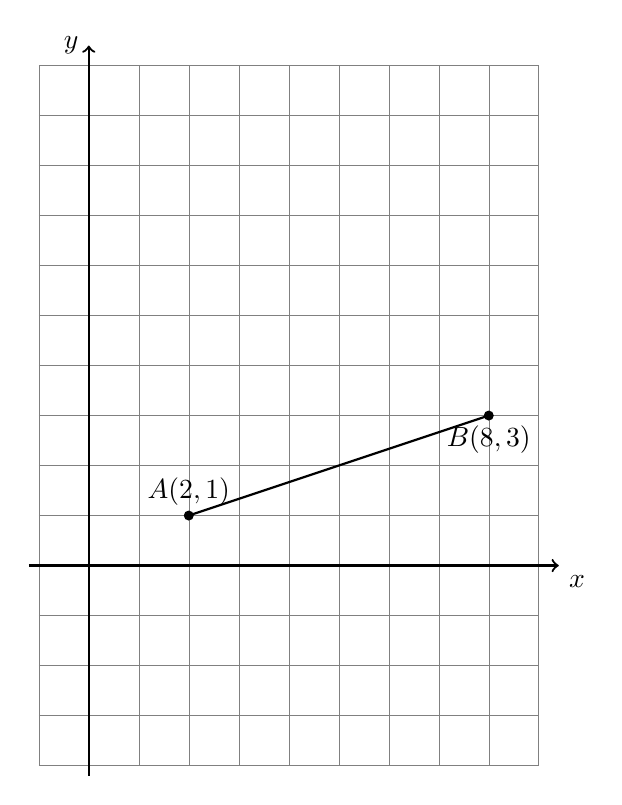
\begin{tikzpicture}[scale=.635]
      \draw [help lines] (-1,-4) grid (9,10);
      \draw [thick, ->] (-1.2,0) -- (9.4,0) node [below right] {$x$};
      \draw [thick, ->] (0,-4.2)--(0,10.4) node [left] {$y$};
      \draw [thick] (2,1)--(8,3);
      \fill (2,1) circle[radius=0.1cm]node[above]{$A(2,1)$};
      \fill (8,3) circle[radius=0.1cm]node[below ]{$B(8,3)$};
    \end{tikzpicture}
    \end{center} 
  \end{multicols}




  
\end{enumerate}
\end{document}
